\chapter{Embedding the Simulation Kernel}
\label{cha:embedding}

\section{Architecture}

{\opp} has a modular architecture. The following diagram shows the
high-level architecture of {\opp} simulations:

\begin{figure}[htbp]
  \begin{center}
    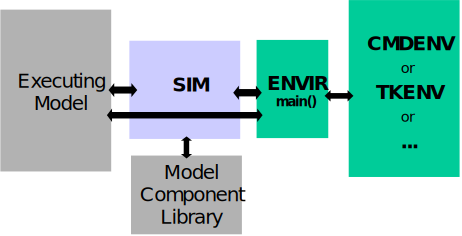
\includegraphics[width=4.757in, height=2.412in]{figures/architecture}
    \caption{Architecture of {\opp} simulation programs}
  \end{center}
\end{figure}

The rectangles in the picture represent components:

\begin{itemize}
  \item{\textbf{Sim} is the simulation kernel and class
    library\index{simulation!kernel}. Sim exists as a library you link
    your simulation program with.}
  \item{\textbf{Envir} is another library which contains all code
    that is common to all user interfaces. \fname{main()} is also in Envir.
    Envir provides services like ini file handling for specific user interface
    implementations. Envir presents itself towards Sim and the executing model
    via the \ttt{ev} facade object, hiding all other user interface internals.
    Some aspects of Envir can be customized\index{customization} via plugin
    interfaces. Embedding {\opp} into applications\index{embedding} can
    be achieved by implementing a new user interface in addition to Cmdenv
    and Tkenv, or by replacing Envir with another implementation of \ttt{ev}
    (see sections \ref{sec:plugin-exts:userinterface} and
    \ref{sec:ch-embedding:embedding}.)}
  \item{\textbf{Cmdenv and Tkenv} are specific user interface
    implementations. A simulation is linked with Cmdenv, Tkenv, or both.}
  \item{The \textbf{Model Component Library} consists of simple module definitions and
    their C++ implementations, compound module types, channels, networks,
    message types and in general everything that belongs to models and
    has been linked into the simulation program. A simulation program is
    able to run any model that has all necessary components linked in.}
  \item{The \textbf{Executing Model} is the model that has been set up
    for simulation. It contains objects (modules, channels, etc.) that
    are all instances of components in the model component library.}
\end{itemize}

The arrows in the figure show how components interact with
each other:

\begin{itemize}
  \item{\textbf{Executing Model $\Leftrightarrow$ Sim}. The simulation kernel
    manages the future events and invokes modules in the executing model
    as events occur. The modules of the executing model are stored
    in the main object of Sim, \fvar{simulation} (of class \cclass{cSimulation}).
    In turn, the executing model calls functions in the
    simulation kernel and uses classes in the Sim library.}
  \item{\textbf{Sim $\Leftrightarrow$ Model Component Library}. The simulation kernel
    instantiates simple modules and other components when the simulation model
    is set up at the beginning of the simulation run. It also refers
    to the component library when dynamic module creation is used.
    The machinery for registering and looking up components in the model
    component library is implemented as part of Sim.}
  \item{\textbf{Executing Model $\Leftrightarrow$ Envir}. The \ttt{ev} object,
    logically part of Envir, is the facade of the user interface towards the
    executing model. The model uses \ttt{ev} to write debug logs (\ttt{ev<<},
    \ttt{ev.printf()}).}
  \item{\textbf{Sim $\Leftrightarrow$ Envir}. Envir is in full command of what
    happens in the simulation program. Envir contains the \ttt{main()} function
    where execution begins. Envir determines which models should be set up
    for simulation, and instructs Sim to do so. Envir contains the main
    simulation loop (\textit{determine-next-event}, \textit{execute-event}
    sequence) and invokes the simulation kernel for the necessary
    functionality (event scheduling and event execution are implemented in Sim).
    Envir catches and handles errors and exceptions that occur
    in the simulation kernel or in the library classes during execution.
    Envir presents a single facade object (\ttt{ev}) that represents
    the environment (user interface) toward Sim -- no Envir
    internals are visible to Sim or the executing model.
    During simulation model setup, Envir supplies parameter values for
    Sim when Sim asks for them. Sim writes output vectors via Envir,
    so one can redefine the output vector storing mechanism by changing Envir.
    Sim and its classes use Envir to print debug information.}
  \item{\textbf{Envir $\Leftrightarrow$ Tkenv/Cmdenv}. Tkenv and Cmdenv
    are concrete user interface implementations. When a simulation program
    is started, the \ttt{main()} function (which is part of Envir) determines
    the appropriate user interface class, creates an instance and runs it
    by invoking its \ttt{run()} method. Sim's or the model's calls on the
    \ttt{ev} object are delegated to the user interface.}
\end{itemize}


\section{Embedding the {\opp} simulation kernel}
\label{sec:ch-embedding:embedding}

This section discusses the issues of embedding the simulation kernel
or a simulation model into a larger application. We assume that you
don't just want to change one or two aspects of the simulator
(like event scheduling or result recording) or create a new user interface
a'la Cmdenv or Tkenv -- if so, see chapter \ref{cha:plugin-exts}.

For the following discussion, we assume that you write the embedding
program from scratch, i.e. starting from a \fname{main()} function.

\subsection{The main() function}

Here's an minimalistic program that initializes the simulation library,
and runs two simulations. In later sections we'll go through details
of the code and discuss how to elaborate it.

\begin{verbatim}
#include <omnetpp.h>

int main(int argc, char *argv[])
{
    // the following line MUST be at the top of main()
    cStaticFlag dummy;

    // initializations
    ExecuteOnStartup::executeAll();
    SimTime::setScaleExp(-12);

    // set up an environment for the simulation
    cEnvir *oldEv = evPtr;
    evPtr = new CustomSimulationEnv();

    // load NED files
    simulation.loadNedSourceFolder("./mysim-core");
    simulation.loadNedSourceFolder("./mysim-ext");
    simulation.doneLoadingNedFiles();

    // set up and run a simulation model
    simulate("FooNetwork", 1000);
    simulate("BarNetwork", 2000);

    // exit
    delete evPtr;
    evPtr = oldEv;
    return 0;
}
\end{verbatim}

The first few lines of the code initialize the simulation library. The
purpose of \cclass{cStaticFlag} is to set a global variable to \ttt{true}
for the duration of the \ttt{main()} function, to help the simulation
library handle exceptions correctly in extreme cases.
\ttt{ExecuteOnStartup::executeAll()} does various startup tasks such as
building registration tables out of the \fmac{Define\_Module()},
\fmac{Register\_Class()} and similar entries throughout the code.
\ttt{SimTime::setScaleExp(-12)} sets simulation time resolution to
picoseconds; other values can be used as well, but it is mandatory to
choose one.

The lines dealing with \ttt{evPtr} set up an environment for the
simulation. \ttt{evPtr} is a global variable behind the \ttt{ev} object;
basically, \ttt{ev} is defined as \ttt{(*evPtr)}. The environment object
contains callback functions invoked by the simulation kernel (and sometimes
model code) to log debug output, access the configuration, record simulation
results and so on. The \ttt{CustomSimulationEnv} class has to be provided by
you; this is discussed in detail in a later section.
Note that \ttt{evPtr} gets restored to its original value at the end
of \ttt{main()}. This is necessary because the \ttt{simulation} object
or other objects may call \ttt{ev} methods in their destructors,
when your \ttt{CustomSimulationEnv} object no longer exists.

The code then loads the NED files from the \ttt{mysim-core} and
\ttt{mysim-ext} subdirectories of the working directory (as if the NED path
was \ttt{./mysim-core;./mysim-ext}), and goes on to run two simulations.


\subsection{The simulate() function}

A minimalistic version of the \ttt{simulate()} function:

\begin{verbatim}
void simulate(const char *networkName, simtime_t limit)
{
    // set up the network
    cModuleType *networkType = cModuleType::find(networkName);
    if (networkType == NULL) {
        printf("No such network: %s\n", networkName);
        return;
    }
    simulation.setupNetwork(networkType); //XXX may throw exception

    // prepare for running it
    simulation.startRun();

    // run the simulation
    bool ok = true;
    try {
        while (simulation.getSimTime() < limit) {
            cSimpleModule *mod = simulation.selectNextModule();
            if (!mod)
                break;  //XXX
            simulation.doOneEvent(mod);
        }
    }
    catch (cTerminationException& e) {
        printf("Finished: %s", e.what());
    }
    catch (std::exception& e) {
        ok = false;
        printf("ERROR: %s", e.what());
    }

    if (ok)
        simulation.callFinish();  //FIXME what if there's an exception during finish()?

    // finish the simulation and clean up the network
    simulation.endRun();
    simulation.deleteNetwork();
}
\end{verbatim}

The function accepts a network type name (which must be fully qualified,
i.e. with package name), and a simulation time limit.

In the first few lines we look up the network name among the modules that
have been loaded from NED files, and print an error message if not found.
Then we set it up as a network. This creates the system module and recursively
all modules and their interconnections; module parameters are also
read from the configuration (where needed) and assigned. If there is
an error (module type not found, etc.), an exception will be thrown.
The exception type is \cclass{std::exception}, usually its
\cclass{cRuntimeError} subclass.

If network setup was successful, we call \ttt{simulation.startRun()}, one
side effect of which is that the \fname{initialize()} methods of modules
and channels get invoked. This step also results in an exception if
something goes wrong in an \fname{initialize()}.

The following lines actually run the simulation, by calling
\ttt{simulation.selectNextModule()} and \ttt{simulation.doOneEvent()} in an
event loop, until the simulation time limit is reached or some exception
occurs. If the exception is a \cclass{cTerminationException} (or subclassed
from it), it signals the normal termination of the simulation; otherwise it
is an error.

If the simulation has completed successfully (\ttt{ok==true}), the code
goes on to call the \fname{finish()} methods of modules and channels.
Then, regardless of whether there was an error, \fname{simulation.endRun()}
has to be called, and the network is torn down with
\fname{simulation.deleteNetwork()}.


\subsection{Providing an environment object}

The environment object needs to implement the \cclass{cEnvir} interface.
There are several methods (see "creating a new user interface")

the easiest way to get started is to subclass it from \cclass{cDummyEnvir}.
\cclass{cDummyEnvir}, which defines all pure virtual methods with either
an empty body, or with a body that throws an \ttt{"unsupported method called"}
exception.

some methods that you surely want to redefine are: \fname{readParameter()}


\subsection{Providing a configuration object}

TODO

\subsection{Loading NED files, and its alternatives}

TODO

you can load dirtrees, single files, and also strings containing NED code



\subsection{The simulation loop}

may build in cpu time limit, progress monitor, interactivity etc

single thread!!  if you want to access the simulation from a separate thread,
you must use locking

simptr gets implemented: then several simulations (sim+envir pairs) may coexist,
but they cannot be run concurrently (due to evptr, simptr and static buffers
used here and there)

animation is to be done via environment object callbacks


\subsection{Assigning module parameters}

catch the \fname{readParameter()} method in \cclass{cEnvir}


\subsection{Extracting statistics from the model}

Two alternative ways:

1. direct C++ calls into the model

   cModule *mod = simulation.moduleByPath("net.server.app");
   App *appMod = dynamic_cast<App *>(mod);
   int packetsSent = appMod->getTotalPacketsSent();

2. or: catch the \fname{recordScalar()} method in \cclass{cEnvir}.
   e.g. store everything (in an std::map or something) and later select

  if (dynamic_cast<>


\subsection{Installing a custom scheduler}

The default event scheduler is \cclass{cSequentialScheduler}. To replace
it with a different scheduler (e.g. \cclass{cRealTimeScheduler} or your
own scheduler class), add a \fname{setScheduler()} call into \ttt{main()}:

\begin{verbatim}
cScheduler *scheduler = new CustomScheduler();
simulation.setScheduler(scheduler);
\end{verbatim}

It is usually not a good idea to change schedulers in the middle of
a simulation, so \fname{setScheduler()} may only be called when
no network is set up.


% --------------------
%
% What you'll absolutely need for a simulation to run is the Sim library. You
% probably do not want to keep the appearance of the simulation program, so
% you do not want Cmdenv and Tkenv. You may or may not want to keep Envir.
% You can keep Envir if its philosophy and the infrastructure it provides
% (\ttt{omnetpp.ini}, certain command-line options etc.) fit into your
% design. Then your application, the embedding program will take the place of
% Cmdenv and Tkenv.
%
% If Envir does not fit your needs (for example, you want the model
% parameters to come from a database not from \ttt{omnetpp.ini}), then you
% have to replace it. Your Envir replacement (the embedding application,
% practically) must implement the \cclass{cEnvir} member functions from
% \ttt{envir/cenvir.h}, but you have full control over the simulation.
%
% Normally, code that sets up a network or builds the internals of a
% compound module comes from compiled NED source.  You may not like the
% restriction that your simulation program can only simulate networks
% whose setup code is linked in. No problem; your program can contain
% pieces of code similar to what is currently generated by nedtool and then
% it can build any network whose components (primarily the simple modules)
% are linked in. Moreover, it is possible to write an integrated environment
% where you can put together a network using a graphical editor and right
% after that you can run it, without intervening NED compilation and
% linkage.
%
%
%
% \section{Sim: the simulation kernel and class library}
%
% There is little to say about Sim here, since chapters
% \ref{cha:simple-modules} and \ref{cha:the-simulation-library},
% and part of chapter \ref{cha:messages} are all about
% this topic. Classes covered in those chapters are documented
% in more detail in the API Reference generated by Doxygen.
% What we can do here is elaborating on some internals
% that have not been covered in the general chapters.
%
% The source code for the simulation kernel\index{simulation!kernel}
% and class library reside in the \ttt{src/sim/} subdirectory.
%
%
% \subsection{The global simulation object}
%
% The global \ttt{simulation} object is an instance of \cclass{cSimulation}.
% It stores the model, and encapsulates much of the functionality
% of setting up and running a simulation model.
%
% \ttt{simulation} has two basic roles:
%
% \begin{itemize}
%   \item{it stores modules of the executing model}
%   \item{it holds the future event set (FES\index{FES}) object}
% \end{itemize}
%
% \subsection{The coroutine package}
%
% The coroutine package is in fact made up of two coroutine
% packages\index{coroutine}:
%
% \begin{itemize}
%   \item A portable coroutine package creates all coroutine stacks
%      inside the main stack. It is based on Kofoed's solution\cite{Kofoed95}.
%      It allocates stack by deep-deep recursions and then plays with
%      \fname{setjmp()} and \fname{longjmp()} to switch from one to another.
%
%   \item On Windows, the Fiber functions (\fname{CreateFiber()},
%      \fname{SwitchToFiber()}, etc) are used, which are part of
%      the standard Win32 API.
% \end{itemize}
%
% The coroutines are represented by the \cclass{cCoroutine}
% class. \cclass{cSimpleModule} has \cclass{cCoroutine} as one a
% base class.
%
% \section{The Model Component Library}
%
% All model components (simple module definitions and their C++
% implementations, compound module types, channels, networks,
% message types, etc.) that you compile and link into a simulation
% program are registered in the Model Component Library.
% Any model that has all its necessary components in the
% component library of the simulation program can be run by that
% simulation program.
%
% If your simulation program is linked with Cmdenv or Tkenv,
% you can have the contents of its component library printed,
% using the -h switch.
%
% \begin{verbatim}
% $ ./fddi -h
%
% {\opp} Discrete Event Simulation  (C) 1992-2004 Andras Varga
% ...
% Available networks:
%   FDDI1
%   NRing
%   TUBw
%   TUBs
%
% Available modules:
%   FDDI_MAC
%   FDDI_MAC4Ring
%   ...
%
% Available channels:
%   ...
% End run of {\opp}
% \end{verbatim}
%
% Information on components are kept on registration lists.
% There are macros for registering components (that is, for adding
% them to the registeration lists):
% \ttt{\fmac{Define\_Module()}}, \ttt{\fmac{Define\_Module\_Like()}},
% \ttt{\fmac{Define\_Network()}}, \ttt{\fmac{Define\_Function()}},
% \fmac{Register\_Class()}, and a few others. For components defined
% in NED files, the macro calls are generated by the NED compiler;
% in other cases you have to write them in your C++ source.
%
% Let us see the module registrations as an example. The
%
% \begin{verbatim}
% Define_Module(FIFO);
% \end{verbatim}
%
% macro expands to the following code:
%
% \begin{verbatim}
% static cModule *FIFO__create(const char *name, cModule *parentmod)
% {
%     return new FIFO(name, parentmod);
% }
%
% EXECUTE_ON_STARTUP( FIFO__mod,
%     modtypes.getInstance()->add(
%        new cModuleType("FIFO","FIFO",(ModuleCreateFunc)FIFO__create)
%     );
% )
% \end{verbatim}
%
% When the simulation program starts up, a new \cclass{cModuleType}
% object will be added to the \ttt{modtypes} object, which holds the list
% of available module types. The \cclass{cModuleType} object will act as a factory:
% when its create() method is called it will produce a new module object
% of class \ttt{FIFO} via the above static function \ttt{FIFO\_\_create}.
%
% The \ttt{cModuleType} object also stores the name of the corresponding
% NED module declaration. This makes it possible to add the gates and parameters
% declared in NED to the module when it is created.
%
% The machinery for managing the registration lists are part
% of the Sim library. Registration lists are implemented
% as global objects.
%
% The registration lists are:
%
% \begin{longtable}{|p{2cm}|p{4,3cm}|p{7.3cm}|}
% \hline
% %% ROW 1
% \tabheadcol
% \textbf{List variable}
% &
% \textbf{Macro/}\linebreak
% \textbf{Objects on list}
% &
% \textbf{Function} \\\hline
% %% ROW 2
% \ttt{networks}
% &
% \ttt{\fmac{Define\_Network()}} \linebreak
% \linebreak
% \ttt{\cclass{cNetworkType}}
% &
% {\raggedright List of available networks\index{network!list of}.
% Every \cclass{cNetworkType} object is a factory for a specific
% network type. That is, a \cclass{cNetworkType} object has methods
% for setting up a specific network.
% \fmac{Define\_Network()} macros occur in the code generated by the NED
% compiler.}\\\hline
% % ROW 3
% \ttt{modtypes}
% &
% \ttt{\fmac{Define\_Module()},} \linebreak
% \ttt{\fmac{Define\_Module\_Like()},}  \linebreak
% \linebreak
% \ttt{\cclass{cModuleType}}
% &
% {\raggedright List of available module types.
% Every \cclass{cModuleType} object is a factory for a specific module
% type. Usually, \fmac{Define\_Module()} macros for compound modules occur in
% the code generated by the NED compiler; for simple modules,
% the \fmac{Define\_Module()} lines are added by the user.}\\\hline
% %% ROW 4
% \ttt{channeltypes}
% &
% \fmac{Define\_Channel()} \linebreak
% \linebreak
% \cclass{cChannelType}
% &
% {\raggedright List of channel types.
% Every \cclass{cChannelType} object acts as a factory for a channel type,
% a class derived from \cclass{cChannel}.} \\\hline
% %% ROW 5
% \ttt{classes}
% &
% \fmac{Register\_Class()} \linebreak
% \linebreak
% \ttt{cClassRegister}
% &
% {\raggedright List of available classes of which one can create
% an instance.
% Every \cclass{cClassRegister} object is a factory for objects
% of a specific class. The list is used by the \fname{createOne()} function:
% it can create an object of any class, given the class name as a string.
% (E.g. the statement \ttt{ptr = createOne("cArray")} creates a \ttt{cArray} object.)
% To enable a class to work with \ttt{createOne()}, one has to register it using the
% \ttt{Register\_Class(classname)} macro}\\\hline
% %% ROW 6
% \ttt{functions}
% &
% \ttt{\fmac{Define\_Function()}} \linebreak
% \linebreak
% \ttt{\cclass{cFunctionType}}
% &
% {\raggedright List of functions taking \ttt{double}s and returning a \ttt{double}
% (see type \ttt{MathFuncNoArg}...\ttt{MathFunc3Args}).
% A \cclass{cFunctionType} object holds a pointer to the function and knows
% how many arguments it takes.}\\\hline
% \end{longtable}
%
%
% \section{Envir, Tkenv and Cmdenv}
%
% The source code for the user interface of {\opp} resides in the
% \texttt{src/envir/} directory (common part) and in the \texttt{src/cmdenv/},
% \texttt{src/tkenv/} directories.
%
% The classes in the user interface are \textit{not} derived from \cclass{cOwnedObject},
% they are completely separated from the simulation kernel.
%
%
% \subsection{The main() function}
%
% The \fname{main()} function of {\opp} simply sets up the user
% interface and runs it. Actual simulation is done in
% \fname{cEnvir::run()} (see later).
%
%
% \subsection{The cEnvir interface}
%
% The \cclass{cEnvir} class has only one instance, a global object
% called \fvar{ev}:
%
% \begin{verbatim}
% cEnvir ev;
% \end{verbatim}
%
% \cclass{cEnvir} basically a facade, its member functions
% contain little code. \cclass{cEnvir} maintains a pointer to a
% dynamically allocated simulation application object (derived from
% \cclass{TOmnetApp}, see later) which does all actual work.
%
%
% \cclass{cEnvir} member functions perform the following groups of tasks:
% \begin{itemize}
%   \item I/O for module activities; the actual implementation is different
%     for each user interface (e.g. stdin/stdout for Cmdenv, windowing
%     in Tkenv)
%   \item cEnvir provides methods for the simulation kernel to
%     access configuration information (for example, module parameter settings)
%   \item cEnvir also provides methods that are called by simulation kernel to
%     notify the user interface of certain events (an object was deleted;
%     a module was created or deleted; a message was sent or delivered, etc.)
% \end{itemize}

%%% Local Variables:
%%% mode: latex
%%% TeX-master: "usman"
%%% End:
